\documentclass[11pt]{scrartcl}
\usepackage{ucs}
\usepackage{float}
\usepackage[utf8x]{inputenc}
\usepackage{ngerman}
\usepackage{amsmath,amssymb,amstext}
\usepackage{graphicx}
\usepackage{tabularx}
\usepackage[square]{natbib}
\usepackage[justification=RaggedRight, singlelinecheck=false]{caption} 
\usepackage{fancyhdr}

\pagestyle{fancy}
\lfoot{Philipp Adler}
\rfoot{\today{}}

\title{Sicherheit}
\author{Philipp Adler}
\date{\today{}}

\begin{document}

\maketitle
\pagebreak
\tableofcontents
\pagebreak

\section{Grundlagen Securityverfahren}
\label{sec:basics-security-process}
% Moderne Kryptographie 2

\subsection{Verschlüsselungsarten}
\label{sec:ciphering types}
Um nicht die eigentliche Nachricht zu übertragen, wendet man einen Schlüssel an, der aus der Nachricht einen sogennannten Chiffretext generiert. Der Empfänger dieses codierten Textes besitzt einen Dechiffrierschlüssel, um die Nachricht in ihren Ursprung zurück zu verwandeln. \grqq{}Dabei kann das Verhältnis zwischen den beiden benutzten Schlüsseln eine von zwei Ausprägungen annehmen, wir sprechen auch von sogenannten Verschlüsselungsarten.\grqq{}\cite{5} Der Standard wäre die symmetrische Verschlüsselung, wo das gleiche Geheimzweichen für das Ver- und Entschlüsseln benutzt wird. Ein Problem beim Austausch des symmetrischen Schlüssel ist, dass Mitlauschen anderer Teilnehmer.\\
Für dieses Problem gibt es eine Lösung, die sogennannte asymmetrische Verschlüsselung. Hier gibt es für das en- und decoding einen eigene Chiffre. Wobei der Verschlüsselungskey für jeden zugänglich ist aber nur der, der den Entschlüsselungkey besitzt, ist in der Lage, die Nachricht zu entschlüsseln. \cite{1}


\section{Symmetrische Verschlüsselung}
\label{sec:symetric-ciphering}
Die Geschichte der symmetrische Verschlüsselung reicht bis in die Antike. Damals wussten nur die Empfänger, nach welchem Verfahren die Botschaft verschlüsselt wurde. Cäsar zum Beispiel verschob jeden Buchstaben um 4 Stellen. Aus diesem Verschlüsselungsalgorithmus entstanden zum einen Blockchiffren und die Stromchiffren. \cite{1}

\subsection{Blockchiffre}
\label{sec:blockchiffre}
% Praktische Kryptographie unter Linux 2.3
% Sicherheit und Kryptographie im Internet 1.4.2
Blockchiffren teilen die Nachricht, die verschlüsselt werden soll, in eine fixe Anzahl an Blöcken, die entweder 64 oder 128 Bit groß sind. Typische bekannte Blockchiffre sind Data Encryption Standard, Advanced Encryption Standard und International Data Encryption Algorithm. \cite{1}
\subsubsection{Der Data Encryption Standard - DES}
\label{sec:data-encryotion-standard}
\grqq{}DES wurde 1977 vom amerikanischen 'National Institute of Standards and Technologies (NIST)' veröffentlicht.\grqq{}\cite{1} Bei diesem Verfahren wird eine Blocklänge von 64 Bit und ein DES-Schlüssel von 56 Bits plus 8 \grqq{}Parity Check Bits\grqq{}\cite{1} eingesetzt. Die ersten 56 Bits werden immer zufällig generiert. Die letzten 8 Bits sorgen dafür, dass keine Übertragungsfehler auftreten. Da 56 Bit zufällig sind, können daraus 2\textsuperscript{56} Schlüsseln erzeugt werden. 16 Runden wird ein Block in einen 64 Bit großen Ausgabeblock umgewandelt. Bei jedem Durchgang wird ein anderer Schlüssel für die Verschlüsselung angwendet. \cite{1}\cite{4}\\\\
\noindent \textbf{Das Schema}\\
Beim Verschlüsselungsverfahren wird der Klartext in Blöcke umgewandelt, welche alle eine Länge von 64 Bit haben, Eingangspermutation IP. Dieser Block wird dann nochmals zerlegt, sodass daraus 2 mal 32 Bit Blöcke entstehen. Der Data Encryption Standard besteht aus 16 Runden. In jeder Runde wird auf der rechten Hälfte ein Verschlüsselungsalgorithmus \textit{f}, die Rundenfunktion, angewendet. Diese werden mit den 32 Bit der rechten Hälfte, die auf 48 Bit expandiert sind, mittels XOR-Gatter verknüpft. Die 32 Bit Blöcke werden in 4 aufgeteilt und bekommen zusätzlich am Rand die Nachbarbit. \cite{2}\\
\begin{figure}[H]
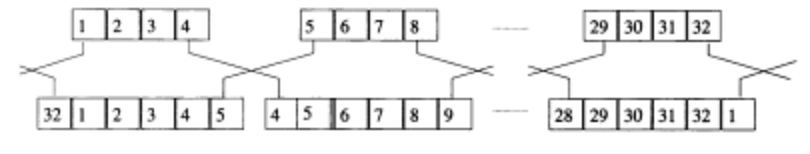
\includegraphics[width=0.60\textwidth]{Bilder/DES/DES_Expansionsabbildung}
	\caption{Expansionsabbildung des DES \cite{2}}
	\label{fig1}
\end{figure}
\noindent \grqq{}Die resultierenden 48 Bits werden in acht Blöcke zu je sechs Bits aufgeteilt\grqq{}\cite{2}, welche als Input für das S-Boxen gebraucht werden. Die Substitution-Box besteht aus einer 4 * 16 Matrix, \grqq{}wobei in jeder Zeile eine Permutation der Zahlen von 0,...,15 steht.\grqq{}\cite{2} Die beiden Randbit der Blöcke entscheiden die Zeile und der Rest, die inneren Bits der Blöcke, die Spalte der Substitution-Box. Die ausgewählte Zahl wird dann binär als 4 Bit Block angegeben. \cite{2}
\begin{figure}[H]
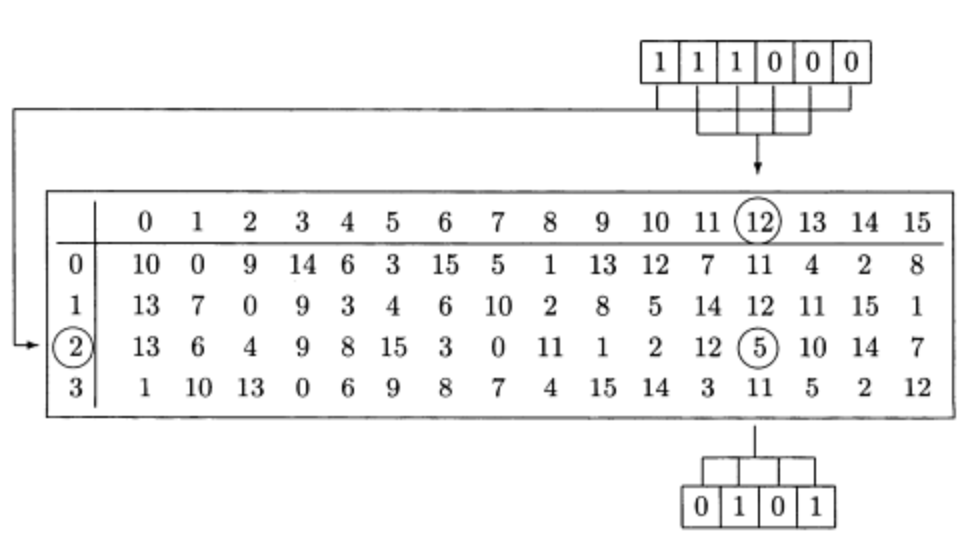
\includegraphics[width=0.45\textwidth]{Bilder/DES/S-Box}
	\caption{S-Box \cite{2}}
	\label{fig2}
\end{figure}
\noindent Da wir nun wieder acht Blöcke zu je 4 Bit haben, können diese zu 32 Bit zusammengefasst werden. \cite{2}
\begin{figure}[H]
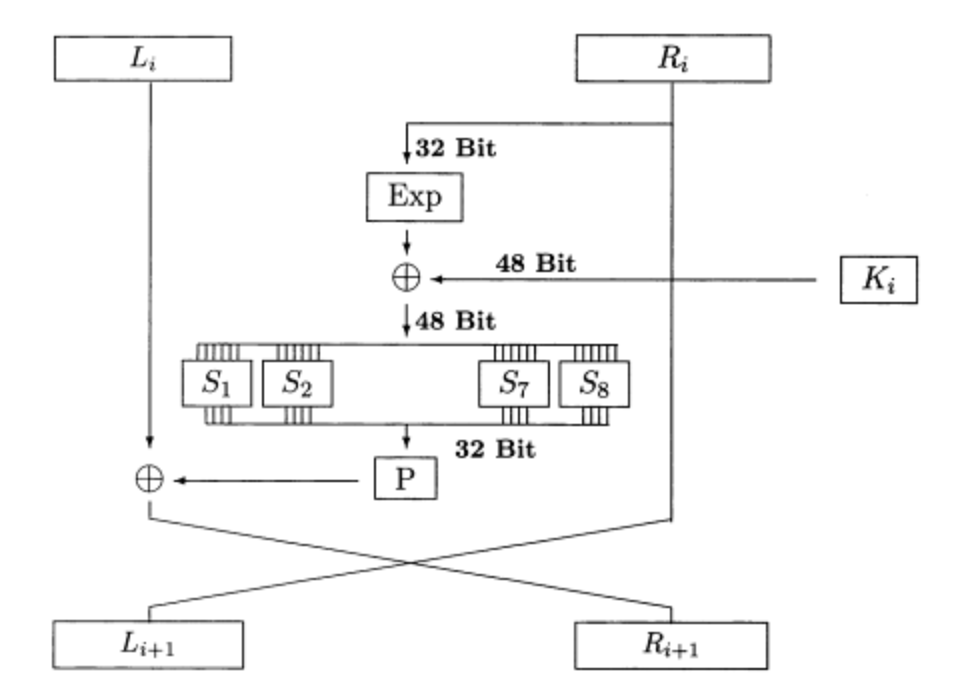
\includegraphics[width=0.45\textwidth]{Bilder/DES/DES_Rundenfunktion}
	\caption{Die DES-Rundenfunktion \cite{2}}
	\label{fig3}
\end{figure}
\noindent Das daraus resultierende Ergebnis wird nochmals permutiert und bitweise mit einem XOR-Gatter mit der linken Hälfte verknüpft. Diese \grqq{}bildet die rechte Seite der neuen Runde.\grqq{}\cite{2} Unter permutieren versteht man, dass jedes einzelne Bit als Zahl dargestellt und mit 8 addiert wird. \cite{2}
\begin{figure}[H]
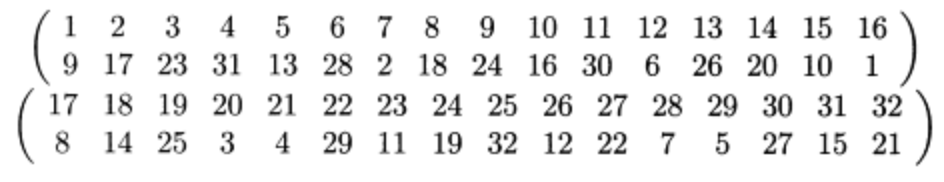
\includegraphics[width=0.40\textwidth]{Bilder/DES/DES_Permutation}
	\caption{Permutation de DES \cite{2}}
	\label{fig4}
\end{figure}
\noindent 
Da der 48 Bit Schlüssel, welcher vom 56 Bit-Hauptschlüssel hergeleitet wird, bei jeder Runde ein anderer ist, muss dieser irgendwie generiert werden. Dazu wird der Hauptschlüssel permutiert. Die Funktion PC-1 teilt diesen in 2 Blöcke zu je 28 Bit. Bei der Permutierung werden die 8 Paritätsbit entfernt, Bits mit der Nummer 8, 16, 24, 32, 40, 48, 56, 64, also bleiben noch 56 Bit übrig. Jede der beiden Hälften wird bei jeder Iteration zirkulärisch links für die Verschlüsselung und nach rechts für die Entschlüsselung gesshiftet. Das heißt, dass jeder Block entweder ein oder zwei Bit nach links rotiert und auf 24 Bit extrahiert wird. So kann es nicht vorkommen, dass ein Rundenschlüssel zweimal angewand wird.\\
\grqq{}Nach 16 Runden werden die 64 Bit einer Ausgangspermutation unterzogen\grqq{}\cite{2}, woraus der Geheimtext resultiert. Die Ausgangspermutation ist die inverse von der Eingangspermutation. Alle 64 Bit Blöcke werden zu einem Geheimtext zusammengeführt. Nachteil dieser Implementierung ist, dass die Ein- und Ausgangspermutation öffentlich sind und so von Angreifern berechnet werden können, was die Sicherheit drastisch verringert. \cite{2}\cite{4}
\begin{figure}[H]
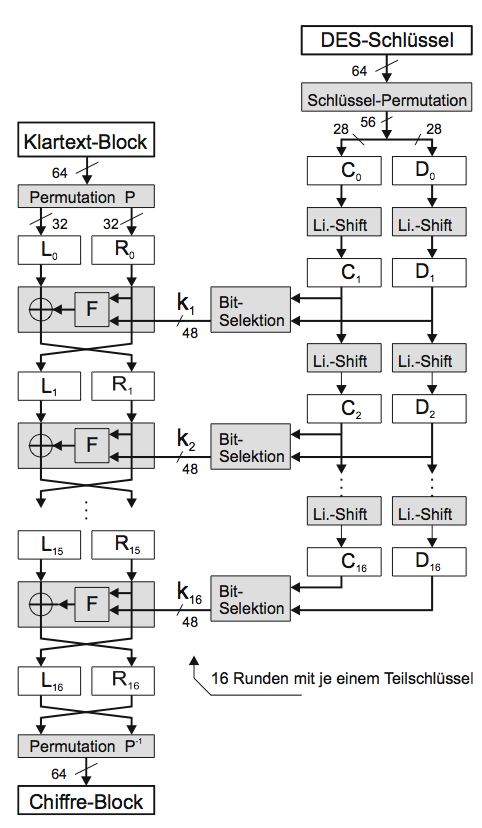
\includegraphics[width=0.30\textwidth]{Bilder/DES/DES_Schema}
	\caption{DES-Verschlüsselung-Schema \cite{3}}
	\label{fig5}
\end{figure}
% Kryptografie in Theorie und Praxis 7.6
% Kryptograhie und IT-Sicherheit 2.2
% Verteilte Systeme S.427

\subsubsection{Der Advanced Encryption Standard - AES}
\label{sec:advanced-encryotion-standard}
Da der DES-Algorithmus aus einen verhältnismäßig kurzen 56-Bit Schlüssel besteht und dieser 1999 durch einen sogenannten Brute-Force-Angriff in 22 Stunden geknackt werden konnte, mussten andere Vorschläge her. Die Alternative hieß AES, Advanced Encryption Standard, ist ebenfalls eine symmetrische Block-Chiffre, mit einer Blocklänge von 128 Bit. \cite{3}\\

\noindent \textbf{Das Schema}\\
Der Unterschied zum DES ist, dass AES eine flexible Block- und Schlüssellänge besitzt. AES besitzt eine Standardmäßige Blocklänge von 128 Bit und Schlüssellängen von 128 Bit, 192 Bit und 256 Bit. Wieviele Runden absolviert werden hängt von der Schlüssellänge ab. Derzeitiger Standard 10 Runden bei einer Schlüssellänge von 128 Bit, 12 Runden bei 192 Bit und 14 Runden bei 256 Bit. \grqq{}Vor der ersten Runde wird ein Rundenschlüssel mit dem Klartext XOR-verknüpft.\grqq{}\cite{2} \cite{3}
\begin{figure}[H]
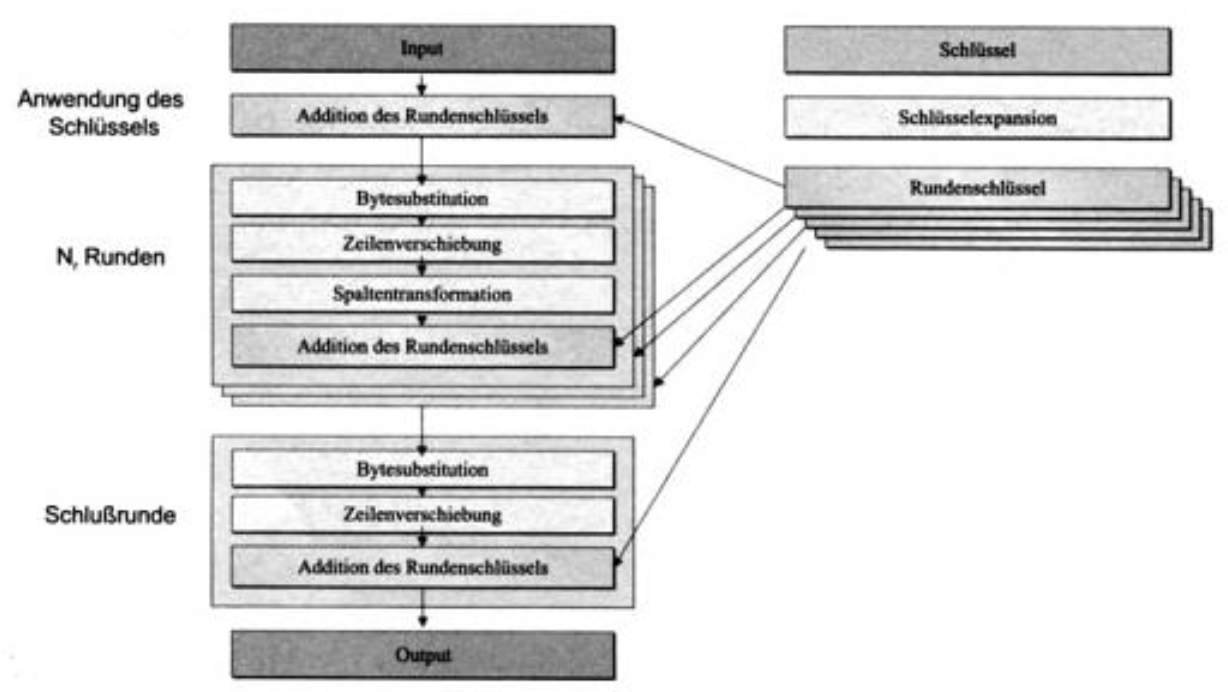
\includegraphics[width=0.55\textwidth]{Bilder/AES/AES_Schema}
	\caption{Schema des AES \cite{3}}
	\label{fig6}
\end{figure}
\noindent 
Beim AES wird der Text und die Ergebnisse als Bytes in einer 4x4-Matrix, in sogenannten States gespeichert. Die Einträge erfolgen spaltenweise, wobei von links nach rechts angeordnet wird. Bei dieser Transformationsfunktion werden die 128 Bit in 16 Bytes geteilt. Die Suche erfolgt mittels der Indexe. \cite{2}\cite{3}
\begin{figure}[H]
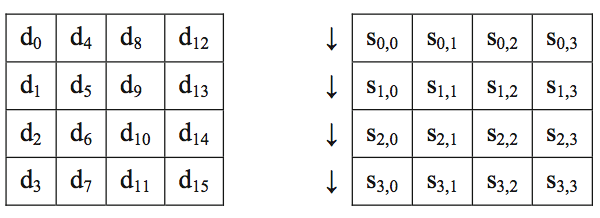
\includegraphics[width=0.40\textwidth]{Bilder/AES/AES_State}
	\caption{Datenstruktur: ein State \cite{3}}
	\label{fig7}
\end{figure}
\noindent
Wie DES eine besitzt auch AES eine Rundenfunktion. Diese besteht aus SubBytes, ShiftRow, MixColumn und AddRoundKey.\\
Beim SubBytes werden die States substituiert. Zuerst wird das Eingangsbyte durch die gebildete Inverse a{\tiny r,c} ersetzt.
\grqq{}Entscheidend für das Verständnis des AES ist, dass die Bytes als Elemente des Körpers \textit{GF}(2\textsuperscript{8}) aufgefasst werden.\grqq{}\cite{2} Dadurch ist es möglich Bytes zu addieren und multiplizieren. Dieser Körper wird durch Polynome in Form als \textit{GF}(2)[\textit{x}]/(\textit{x}\textsuperscript{8} + \textit{x}\textsuperscript{4} + \textit{x}\textsuperscript{3} + \textit{x} + \textit{1}) dargestellt. Für die Berechnung wird das Byte in Bits dargestellt und einem Polynom zugeordnet. Es wird dann nur mehr mit Polynomen gerechnet. \textit{{10100010} = x\textsuperscript{8} + x\textsuperscript{6} + x}\\
Der neue State wird mit einer 8x8 Matrix mod 2 multipliziert. Daraus ergibt sich ein Byte großer Ergebnisvektor, der zum Schluss mit der Konstante GF(2\textsuperscript{8}) addiert wird. Vorteil an diesem Algorithmus ist, dass die Bildung der Inverse eines Bytes nicht-linear ist, was jedoch die Analyse des AES erschwert. \cite{2}\cite{3}\\
\begin{figure}[H]
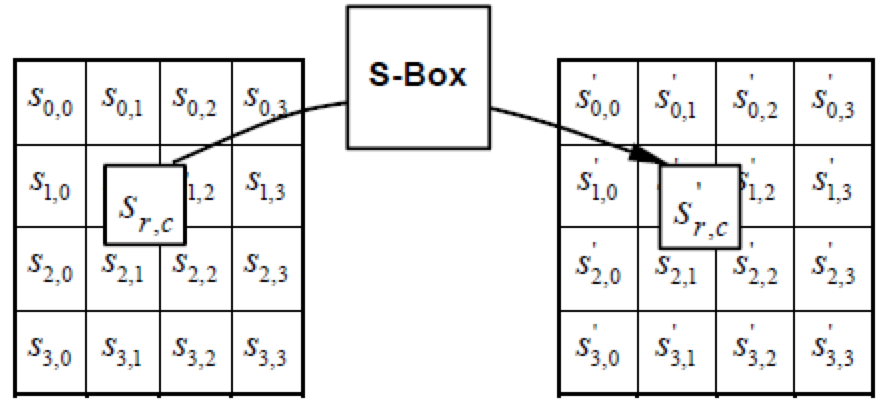
\includegraphics[width=0.40\textwidth]{Bilder/AES/AES_SubBytes}
	\caption{Die Abbildung SubBytes \cite{2}}
	\label{fig8}
\end{figure}
\noindent
ShiftRow und MixColumn stellen die Permutation der Rundenfunktion dar, wobei ShiftRow zeilenweise operiert und MixColumn spaltenweise. Beim ShiftRow besteht die Permutation aus einem Linksshift, der von der Blocklänge abhängig ist. Ausgenommen ist die erste Zeile, weil diese nie verschoben wird. Ansonsten wird die 2.Zeile um C1 Bytes, die 3.Zeile um C2 und die 4.Zeile um C3 Bytes verschoben. Falls die Blocklänge 128 Bit beträgt, wird wie folgt nach Links geshiftet. \cite{2}
\begin{figure}[H]
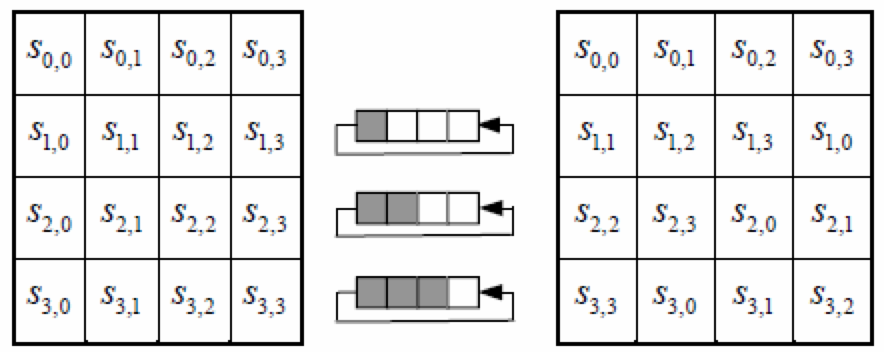
\includegraphics[width=0.40\textwidth]{Bilder/AES/AES_ShiftRow}
	\caption{Die Abbildung ShiftRow \cite{2}}
	\label{fig9}
\end{figure}
\noindent
Wie schon oben erwähnt kümmert sich der MixColumn um die Spalten, welche aus 4 Byte bestehen, die wie bei SubBytes als Polynom dargestellt werden. Da wir hier nur 4 Byte haben, ist der Grad kleiner gleich 3. Das daraus erzeugte Polynom wird mit einer Konstante mod (x\textsuperscript{4} + 1) multipliziert. \cite{2}
\begin{figure}[H]
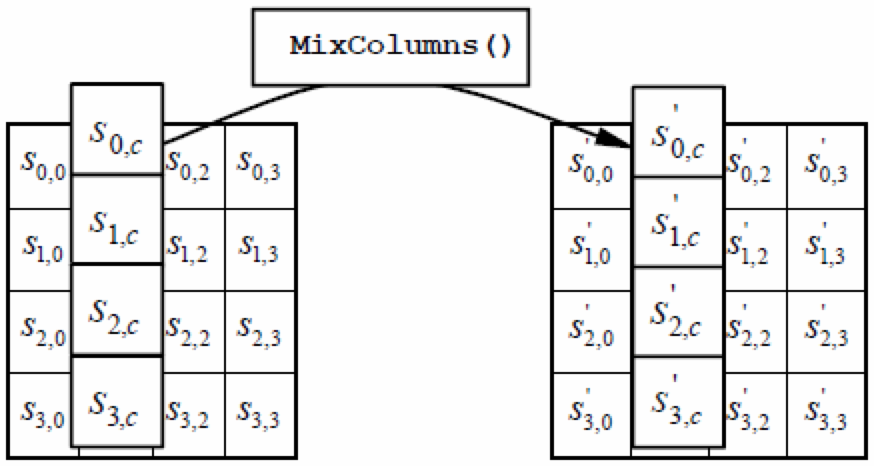
\includegraphics[width=0.40\textwidth]{Bilder/AES/AES_MixColumn}
	\caption{Die Abbildung MixColumn \cite{2}}
	\label{fig10}
\end{figure}
\noindent
AddRoundKey wird zu Beginn und am Ende jeder Runde eingesetzt, um den aktuelle Rundenschlüssel und den Block mittels einer XOR-Verknüpfung zu addiert. Der Rundenschlüssel wird durch die Formel (Rundenanzahl + 1) * (Anzahl der Wörter pro Matrix) hergeleitet. Da bei 128 Bit mehr Bits zur Verfügung stehen als benötigt werden, muss der Schlüssel expandiert werden. Bei der Expansion wird der externe Schlüssel in seine Bestandteile zerlegt, im Falle von 128 Bit sind es 4 Wörter. Dabei wird i und i+3 mittels XOR verknüpft.\\
In jeder neuen Runde werden andere Rundenschlüssel verwendet. Man verwendet in der Ersten die ersten vier Wörter und in den nächsten die nächsten vier. \cite{2}

% Kryptografie in Theorie und Praxis 7.7
% Kryptograhie und IT-Sicherheit 2.6

% Moderne Kryptographie 4.5

\subsubsection{IDEA (International Data Encryption Algorithm)}
\label{sec:international-data-encryption-algorithm}
Der International Data Encryption Algorithm ist ebenfalls wie DES und AES eine symmetrische Block-Chiffre. Sie besteht aus einer Blocklänge von jeweils 64 Bit und einer Schlüssellänge von 128 Bit. \cite{3}\\

\noindent \textbf{Das Schema}\\
Das IDEA besteht aus 9 Runden, die ersten 8 Runden führen alle den gleichen Vorgang aus. Der Klartext, bestehend aus 64 Bit wird in 4 Blöcke aufgespalten. Der erste und letzte Block wird mit einem Teilschlüssel modulo (2\textsuperscript{16} + 1) multipliziert, weil immer ein Rest auftritt, da es sich um eine Primzahl handelt. Die inneren Blöcke werden stattdessen modulo (2\textsuperscript{16}) addiert. In der Mitte des Schemas werden 2 andere Teilschlüssel eingesetzt, welche die Ergbnisse von oben addieren oder multiplizieren. Am Ende jeder Runde werden die innen Ausgänge vertauscht. Da in jeder Runde ein anderer Klartext zum Einsatz kommt, werden auch andere Teilschlüssel angewandt. \grqq{} Aus den Primärschlüssel werden 52 Teilschlüssel von 16 Bit Länge erzeugt, von denen je sechs in acht Runden zum Einsatz kommen.\grqq{}\cite{6}
Nach den ersten 8 Runden, kommen wir nun zur letzten, der 9ten Runde, in der der Hauptteil des Verschlüsselungsschemas ausgelassen wird. Dagegen werden 4 Teilschlüssel k{\scriptsize 9,1}, k{\scriptsize 9,2}, k{\scriptsize 9,3}, k{\scriptsize 9,4} eingesetzt. \cite{3}\cite{6}
\begin{figure}[H]
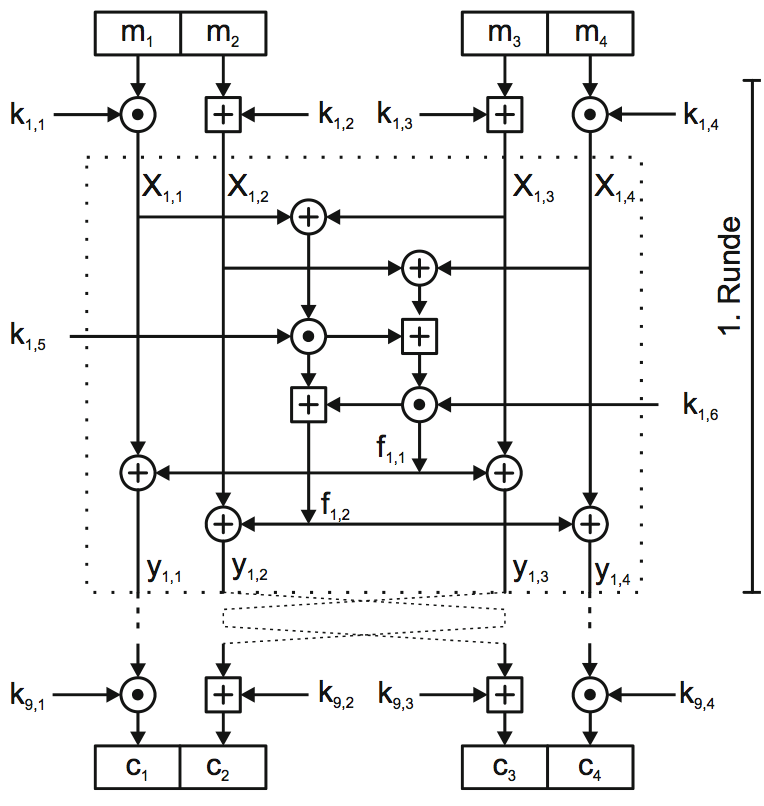
\includegraphics[width=0.40\textwidth]{Bilder/IDEA/IDEA_Schema}
	\caption{IDEA Schema \cite{3}}
	\label{fig11}
\end{figure}
\noindent
Die Entschlüsselung funktioniert wird die Verschlüsselung nur umgekehrt in die andere Richtung. Die Teilschlüssel k{\scriptsize 9,x} werden invertiert. \cite{3}
% Kryptograhie und IT-Sicherheit 2.3

\section{Asymmetrische Verschlüsselung}
\label{sec:asymetric-ciphering}

\subsection{Der RSA-Algorithmus}
\label{sec:rsa-algorithmus}
Eines der bekanntesten Public-Key-Verfahren ist der RSA-Algorithmus. Entwickelt wurde es 1977 von Rivest, Shamir, Aleman. Das Verfahren beruht auf der Schwierigkeit der Faktorisierung von Zahlen, der sogenannte Satz von Euler. Beim RSA wird ein Nachrichtenblock als Zahl interpretiert, welche kleiner als modula \textit{n} ist. \cite{2}
% 6.Praktische Kryptographie unter Linux 2.4.3
% 2.Kryptografie in Theorie und Praxis 10
% 3.Kryptograhie und IT-Sicherheit 4.2
% 5.Moderne Kryptographie 6.4
% 1.Sicherheit und Kryptographie im Internet 1.5.4

\subsubsection{Schlüsselerzeugung}
\label{sec:key-generation}
Für die Erzeugung des Schlüssels \textit{n} benötigt man das Produkt von zwei Primzahlen \textit{p} und \textit{q}, die mindestens 512 Bit lang sind 2\textsuperscript{512} und geheim sind. Die Wahrscheinlichkeit, dass es sich um eine Primzahl handelt ist 2\textsuperscript{-9}. Um das faktorisieren zu erschweren gibt es spezielle Faktoren. Erstens die Primzahlen sollten sich nicht zu sehr unterscheiden, aber auch nicht beieinander liegen. Für die Teilfremdezahl sollte man möglichst kleine Teiler haben. Als nächstes wird eine Zahl \textit{e}, enciphering, die teilfremd zu $\varphi(n)$ = (p - 1)(q - 1) ist, ausgewählt. Unter Teilfremd versteht man, dass beiden Zahlen keinen gemeinsamen Teiler haben. Mit diesen Zahlen wird der öffentliche Schlüssel (\textit{e, n}) gebildet. Damit der Empfänger die Nachricht entschlüsseln kann, benötigt er den privaten Schlüssel \textit{d}. Die Zahl \textit{d} wird mit Hilfe des Euklidischen Algorithmus \textit{e * d mod (p - 1)(q - 1) = 1} berechnet.\\\\
\noindent\\\\
\textbf{RSA-Signatur}\\
\grqq{}Mit Hilfe des RSA-Verfahrens kann man leicht eine digitale Signatur realisieren: Man bildet zunächst den Hashwert \textit{h = hash(m)}, der zu signierenden Nachricht \textit{m}, und berechnet die Signatur, indem man diesen Hashwert 'entschlüsselt'.\grqq{}\cite{1}
Um die Signatur zu prüfen, wird der Hash des Dokuments nochmals gebildet und \grqq{} dann der Wert \textit{sig} durch Potenzierung mit dem öffentlichen Schlüssel \textit{e} 'entschlüsselt'.\grqq{}\cite{1}.
Wenn beide übereinstimmen, war die Signatur korrekt. \cite{1}\cite{2}\cite{6}
\subsubsection{Verschlüsseln}
\label{sec:rsa-encrypt}
Bei der Verschlüsselung wendet der Sender den öffentlichen Schlüssel des Empfängers. \textit{c} = \textit{m}\textsuperscript{e} (mod \textit{n}) \cite{6}

\subsubsection{Entschlüsseln}
\label{sec:rsa-decrypt}
Der Empfänger muss nur noch seinen privaten Schlüssel auf den Geheimtext \textit{c} zum Entschlüsseln anwenden. \textit{m} = \textit{c}\textsuperscript{d} (mod \textit{n}) \cite{6}

\section{SSL/TLS-Protokoll}
\label{sec:ssl/tls-protocol}
% Praktische Kryptographie unter Linux 8.1
% 3.Kryptograhie und IT-Sicherheit 6.3
% 1.Sicherheit und Kryptographie im Internet 7.7/7.9

\subsection{SSL/TLS Grundlagen}
\label{sec:ssl-tls-basics}
Netscape hat Mitte 1994 die erste Version von SSL(Secure Sockets Layer), für die sichere Kommunikation im WWW, zur Verfügung gestellt. Aufgrund der Verfügbarkeit eines gesicherten TCP Dienstes wurde es möglich, vertrauliche Informationen zu übertragen. \grqq{}Die Internet Engineering Task Force übernahm dann die Aufgabe, SSL zu standardisieren, und brachte 1999 die standardisierte Version TLS 1.0 (Transport Layer Security) heraus.\grqq{}\cite{6} TLS 1.0 zeigt kaum Unterschiede zu SSL 3.1. Der Vorteil an SSL 3.1 im Gegensatz zu 2.0 ist, dass Schwächen wie Fehler im Zufallszahlengenerator odee Angriffe, wie man-in-the-middle, beseitigt wurden. Der Secure Sockets Layer unterstützt außerdem verschieden Kryptoalgorithmen, die zwischen dem Verbindungsaufbau zwischen Client und Server zum Einsatz kommen. \cite{1}\cite{3}\cite{6}

\subsection{SSL/TLS im Protokollstapel}
\label{sec:ssl-tls-protocolstack}
Wenn wir das OSI-Schichtenmodell betrachten sehen wir, dass sich zwischen Layer 4, TCP/IP und der Anwndungsschicht SSL/TLS befindet. Mit SSL möchte man eine weitere Protokollschicht, eine Verschlüsselungsschicht einbeziehen. Diese Schicht, Record Layer genannt, kümmert sich darum, dass die zu übertragenen Daten verschlüsselt und auf der Empfängerseite entschlüsselt werden. SSL selbst besteht aus 4 Protokollen, SSL-Alert, SSL-Record, SSL-Handshake und SSL-Change-Cipher-Spec.\\
Falls es bei der Kommunikation zu einen Fehlern kommt, teilt dies das SSL Alert-Protokoll den Endusern mit. Das Prokoll besteht aus 2 Byte, wobei das erste Byte den Fehlergrad angibt, warning oder fatal, und das zweite Byte den Fehler beschreibt. Es gibt zwei Gruppen, die close-notify-Nachricht und den Rest. \cite{1}\cite{6}
\begin{figure}[H]
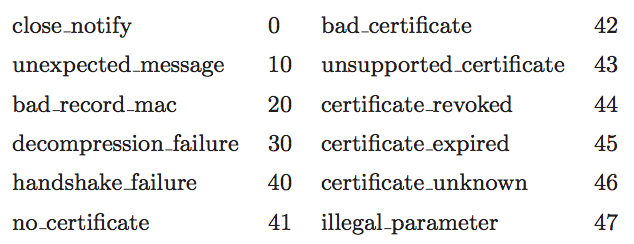
\includegraphics[width=0.40\textwidth]{Bilder/TLS/SSL-Alert}
	\caption{SSL-Alert Beschreibungen \cite{1}}
	\label{fig12}
\end{figure}
\noindent
SSL-Record stellt die verschiedenen Algorithmen unter anderem, MD5 symetrische Verschlüsselung, für den reibungslosen Ablauf zur Verfügung. Wie schon erwähnt ist der SSL Record Layer eine zusätzliche Schicht oberhalb des TCP/IP Layer. Auch er nimmt Byteströme entgegen, welche fragmentiert, in sogenannte \textit{Records}, geteilt und komprimiert werden. Die Recordsgröße wird minimiert, werden. Als nächstes folgt die Authentifizierung durch den Message Authentication Code (MAC), welcher nur von Kommunikationspartnern überprüft werden kann. \grqq{}Bei der anschließenden Verschlüsselung ist zu beachte, dass bei Verwendung einer Blockchiffre die Länge des Klartextes eine Vielfaches der Blocklänge der Chiffre sein muss.\grqq{}\cite{1} Da kommt Padding ins Spiel. Es hängt zusätzliche Bytes an, welche bei der Übertragung mit angegeben werden müssen. Nun muss nur noch \textit{Encrypt} eingesetzt werden, welches den Record verschlüsselt. \cite{1}
\begin{figure}[H]
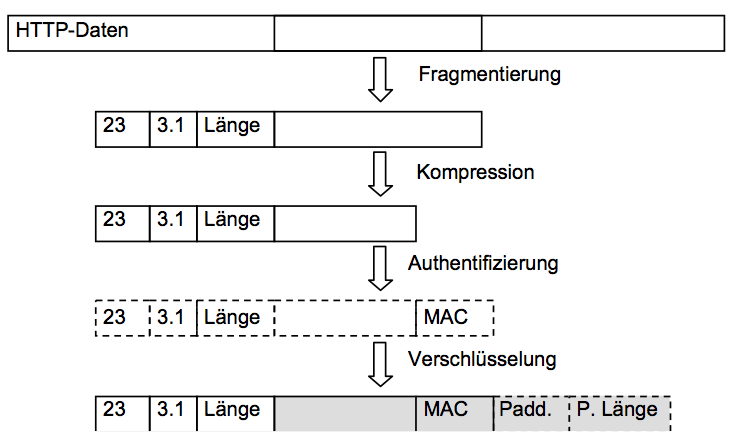
\includegraphics[width=0.40\textwidth]{Bilder/TLS/SSL-Record}
	\caption{SSL Record Layer-Protokoll \cite{1}}
	\label{fig13}
\end{figure}
\noindent
Die zur Auswahl stehenden Protokolle werden beim SSL-Handshake vor der Kommunikation zwischen Client-Server ausgehandelt. Genauere Details erfahren sie in den nächsten Kapiteln.\\
\grqq{}Das SSL-Change-Cipher-Spec-Protocol bereitet die ausgehandelten Protokolle vor bzw inizialisiert Sie.\grqq{}\cite{6}
\cite{6}
\begin{figure}[H]
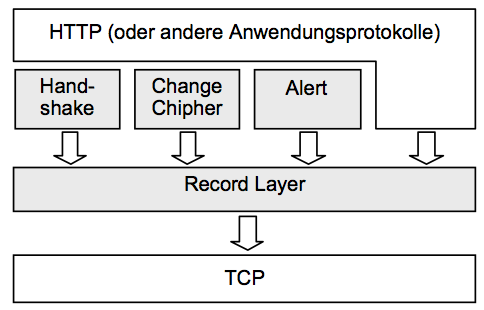
\includegraphics[width=0.30\textwidth]{Bilder/TLS/SSLTLS-TCPIP}
	\caption{Bestandteile des SSL-Protokolls \cite{1}}
	\label{fig14}
\end{figure}

\subsection{SSL-Handshake}
\label{sec:ssl-handshake}
Wie schon oben erwähnt, besteht SSL aus 2 Schichten. Der wichtigste Teil ist das SSL Handshake, wo der zu verwendende Algorithmus bestimmt wird, die Authentifkation und Schlüssel ausgetauscht werden. Es ermöglicht sozusagen die verschlüsselte Kommunikation. 
Die Serveranfrage beginnt mit einer \textbf{client-hello-Nachricht}, es gibt an welche Algorithmen, Ciphersuites, und SSL-Version verwendet werden sollen, damit eine Session-ID erstellt wird. Die Version besteht aus 2 Byte. Hier wählt der Client ob er TLS 1.0 oder TLS 1.1 anwenden will. Falls von einer früheren Sitzung eine Session-ID bekannt ist, verkürzt diese den Handshake Ablauf. Grund dafür ist die Minimierung der Anzahl der Public-Key Operationen. \grqq{}Außerden sendet der Client eine Zufallszahl ClientRandom, die später in die Berechnung der krypographischen Schlüssel mit einfließt.\grqq{}\cite{1}
Die Zufallszahl besteht aus 32 Byte, wobei 4 Byte die Sekunden seit 1.Januar 1970 sind und die restlichen 28 Byte Zufallswerte sind. Beim dem Algorithmus muss mindestens ein symmetrisches Verfahren und Hash-Algorithums für den Schlüsselaustausch gewählt werden, dass kann z.B. RSA und DES sein. \cite{1}
\begin{figure}[H]
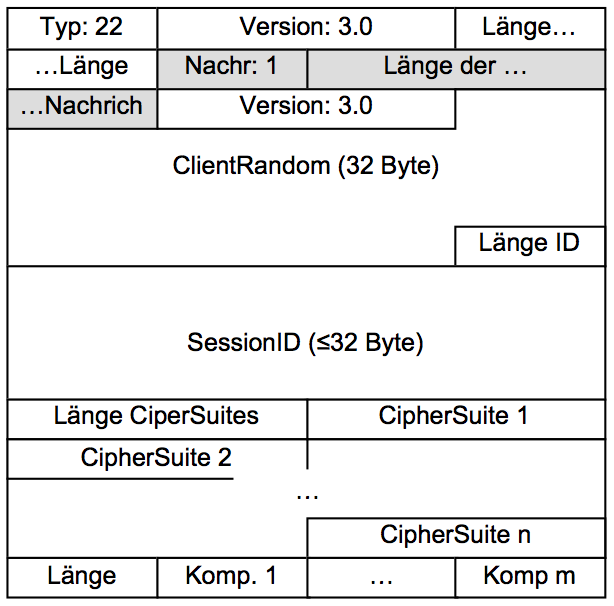
\includegraphics[width=0.40\textwidth]{Bilder/TLS/ClientHello}
	\caption{Die ClientHello-Nachricht \cite{1}}
	\label{fig16}
\end{figure}
\noindent
Der Server anwortet mit einer \textbf{server-hello-Nachricht}, welche einen Algorithmus von der Ciphersuite, eine Reihe von Zufallszahlen ServerRandom und ein \textbf{Zertifikat}, welches seinen öffentlichen und einen privaten Schlüssel, enthält. Die Zufallszahlen werden analog zum den Client-Zufallszahlen gebildet. Es kann vorkommen, dass der Client eine SessionID überträgt, aber nur dann, wenn schon vorher eine Sitzung zwischen den Beiden erstellt wurde. Falls ein Feld leer ist, erzeugt der Server eine neue ID, andernfalls wird die Alte weiterverwendet. Wenn das Zertifikat keinen Schlüssel enthält, muss dieser mittls \textbf{ServerKeyExchange} übertragen werden. Da dies sicherheitskritisch ist, muss dies vom Server signiert werden. Die Response wird mit einen ServerHelloDone beendet.\\
Bevor der Client ein Master Secret erstellt, muss überprüft werden, ob das Zertifikat noch gültig ist, vertrauenswürdig und ob der Domainname mit dem Server-Zertifikat ident ist. Bei positiven Ergebnis, verschlüsselt der Client mit dem öffentlichen Schlüssel des Servers einen geheihmen Wert, 46 Byte langen Zufallszahlen mit 2 Byte Versionsnummer, Premaster Secret und sendet es ihm mittels \textbf{ClientKey-Exchange}. Aus dem Premaste Secret wird dann das Master Secret mittels Hashfunktionen abgeleitet, mit dem man die Sitzungsschlüssel erzeugen kann. Mit \textbf{ChangeCipherSpec} können beide dem Anderen dies mitteilen. Ab sofort werden alle Nachrichten mit dem ausgehandelten Key verschlüsselt.\\
Der Server entschlüsselt die Nachricht, benutzt ebenfalls Hashfunktionen um den Schlüssel zu erzeugen und beendet mit Finished. \cite{1}\cite{6}
\begin{figure}[H]
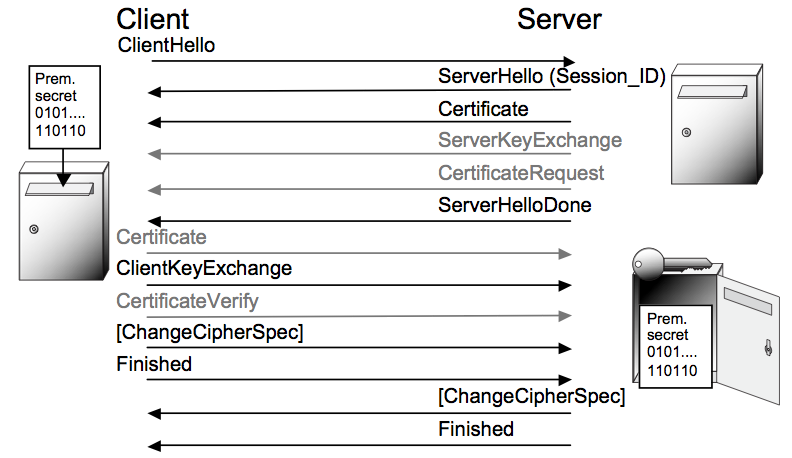
\includegraphics[width=0.40\textwidth]{Bilder/TLS/SSL-Handshake}
	\caption{SSL-Handshake \cite{1}}
	\label{fig16}
\end{figure}

\subsection{TLS Verschlüsselung}
\label{sec:tls-encryption}
% Suchbegriff tls symmetric encryption
% https://info.ssl.com/tls-handshake/
% https://www.digicert.com/ssl-cryptography.htm
% https://technet.microsoft.com/en-us/library/cc781476(v=ws.10).aspx
%  Allgemein und dann auf TLS bezogen

\textbf{Symmetrische Verschlüsselung}\\
Bei dem symmetrischen Verschlüsselungssystem gibt es nur einen Schlüssel, den sogenannten Geheimschlüssel, welcher für die Ver- und Entschlüsselung verwendet wird. Es wird vorrausgesetzt, dass Sender und Empfänger den gleichen Schlüssel für die Kommunikation besitzen. Dieser Schlüssel K{\scriptsize A,B} muss, um die Sicherheit zu gewährleisten, geheimgehalten werden. Verschlüsselungsalgorithmen werden in die zwei Gruppen Blockchiffren und Stromchiffren aufgespalten. Die Schlüssel sind nur 128 oder 256 Bits groß, was ihn schneller als die Asymmetrische Verschlüsselung macht. Probleme bei diesen Scenario, könnte die Verteilung des Schlüssels sein. \cite{4}\\

% 1\ 1.4.1
% 3\ 1.3.2
% Tannenbaum 426
\noindent
\textbf{Asymmetrische Verschlüsselung}\\
Der SSL Handshake verwendet die asymmetrische Verschlüsselung. In diesem System sind die Schlüssel unterschiedlich und bilden zusammen ein eindeutiges Paar. Es gibt zwei Typen von Schlüsseln für die Ver- und Entschlüsselung. Der eine ist public, also von jeden sichtbar, wird durch ein Zertifikat verschickt, und zur Verschlüsselung benutzt, der Andere ist private und nur ein passender Schlüssel kann die Nachricht entschlüsseln. Verschlüsselungsverfahren wären z.B. RSA und ElGamal. Die Schlüssel sind typerischerweise 1024 oder 2048 Bits groß. \cite{4}\\

% 1/ 1.5.1
% 3\ 1.3.3
% Tannenbaum 426


\noindent
\textbf{Hybride Verschlüsselung}\\
Da die Ver- und Entschlüsselung beim asymmetrischen Verfahren zeitaufwändig ist, verwendet man stattdessen das hybride Verfahren. Bei der hybriden Verschlüsselung, wird der symmetrische Schlüssel, zufällig generiert, durch den Public Key vom asymmetrischen Verfahren verschlüsselt. Der zu übertragenede Nachrichtenblock wird mit dem symmetrischen Schlüssel verschlüsselt. Diese Art nennt man hybride Verschlüsselung, da beide Verschlüsselungsarten übertragen werden. Ein Vorteil, die Daten werden schnell und effizient übertragen. Durch das Aymmetrische wird der Key sicher zum Kommunikationspartner übermittelt. Mögliche Algorithmen wären RSA-AES-Verschlüsselung. \cite{3}\\\\
% 1/ 1.5.7
% 1/ 5.2
% 5/ 6.6
% Tannenbaum 426
\noindent
\textbf{Verschlüsselungsalgorithmen}\\
Zum Ableiten von Master Secret aus Premaster Secret, benötigen wir die Pseudozufallsfunktion (PRF). PRF besteht zum einen aus MD5 und zum anderen SHA-1, welche beide Hashfunktionen sind. TLS-PRF besteht aus drei Werten, dem secret, welches aus zwei Teilen besteht die als Input für die zwei Hashfunktionen verwendet wird,  dem label, ein bekannter Wert und seed ein unverschlüsselter Wert der übertragen wird. \grqq{}Die Eingabe label und seed werden dagegen zu einem Wert zusammengefasst.\grqq{}\cite{1} Die Bitströme von den Hashfunktionen werden mit XOR verknüpft, wobei MD5, 128 Bit, fünf mal iteriert wird und SHA-1, 160 Bit, vier mal iteriert. Daraus resultiert ein 640 Bit großer Output. \cite{1}
% https://technet.microsoft.com/en-us/library/cc781476(v=ws.10).aspx
% https://www.digicert.com/ssl-cryptography.htm

\section{Schwierigkeiten bei Software}
\label{sec:sw-trouble}

\subsection{Buffer Ovrflow}
\label{sec:buffer-overflow}
Einem Buffer ist nur ein begrenzter Speicher zugewiesen. Ein Buffer Overflow tritt auf, wenn ein Programm versucht mehr Daten in den Speicher zu schreiben als vorhanden ist. Das kann auftreten, wenn die Übergabelänge nicht überprüft wurde. Die zusätzliche nicht gespeicherte Information, überschreibt gültige Daten. Bei dieser Attacke versucht der Angreifer seinen eigenen Code oder spezielle Prozesse auszuführen. \cite{9}
% 8. Improving Intrusion Detection Systems 4.3
% 9. Network Intrusion Detection and Prevention 1.3.1

\subsection{OpenSSL}
\label{sec:openssl}
OpenSSL ist die am häufigsten eingesetzte TLS-Bibliothek. Doch ist die Bibliothek nicht fehlerfrei. Wir werden uns 3 Angriffscenarien anschauen.\\\\
\noindent
\textbf{Angriff auf den TLS-Handshake}\\
Der Heartbleed ist ein Angriff, bei dem alle Daten von dem TLS-Server ausgelesen werden konnten. Grund dafür war eine Fehlimplementierung in der Heartbeat-Funktion, die auf TLS over UDP ausgelegt ist. Um zu kontrollieren ob der Kommunikationspartner noch aktiv ist, schickt der Server eine Anfrage, beidem vom Partner eine 5 Zeichen große Antwort, nähmlich 'Hello', gefordert ird. Um vom Server geheime Daten zu erhalten, sendet der Angreifer einen Response, wo der Server aufgefordert wird z.B. 55.555 Zeichen zurückzusenden. Er bekam nicht nur das Hello, sondern weitere 55.550 Bytes. Erst eine Neucompilierung des Sourcecodes, beseitigte den Fehler.\\\\
\noindent\\\\
\textbf{Angriff auf den Handshake}\\
Beim Bleichenbacher Angriff handelt es sich um eine Seitenkanal-Attacke. Diese nutzt Information, um eine Analyse des kryptischen Verfahren zu betreiben. Man fängt den ClientKeyExchange, mit der RSA codierten Nachricht, ab und sendet es an den angreifenden Server. Der Server entschlüsselt die Nachricht und überprüft die ersten zwei Byte, die entweder eine Alert Meldung 1 werfen. Wenn die ersten zwei Byte nicht 0x00 0x02 sind oder eine zweite Fehlermeldung geworfen wird, hilft das dem Angreifer das suchende Intervall Premaster Secret zu verkleinern, bis nur noch eine Zahl übrigbleibt. Durch Softwareanpassung in den Frameworks, wurde die Software optimiert.\\\\
\noindent
\textbf{Angriff auf Zertifikate}\\
Häcker verschafften sich Zugang zu einen Rechner, der Zertifikate freigibt. Mehr als 500 Zertifikate wurden ausgestellt, die Hörzwecken dienen sollten. \grqq{}Da jede CA, die in einem Browser mit einem Wurzelzertifikat vertreten ist, SSL-Zertifikate für alle Domains ausstellen kann, wird immer wieder die Vermutung geäußert, dass einige dieser CA auch Zertifikate zu Abhörzwecken ausstellen könnten.\grqq{}\cite{1} Die Behauptungen wurden bis heute nicht belegt. \cite{1}
% 6. Praktische Kryptographie unter Linux 8.2
% 1. Sicherheit und Kryptographie im Internet 7.10

\newpage
\listoffigures
\addcontentsline{toc}{section}{Abbildungsverzeichnis}
\addcontentsline{toc}{section}{Literaturverzeichnis}
\mbox{}
\nocite{*}
\bibliographystyle{unsrt}
\bibliography{literatur}

\end{document}